\chapter{Framework Design}
\label{chap:fw-design}
\index{Framework Design}

%%%%%%%%%%%%%%%%%%%%%%%%%%%%%%%%%%%%%%%%%%%%%%%%%%%%%%%%%%%%%%%%%%%%%%%%%%%%%%%%

In this chapter, we are going to describe the design of our proposed solution
which can fulfill the requirements.
We will first explain why we choose the framework solution. Then we outline the 
architecture of our solution. Finally, we detail each component for both the 
core and specialized frameworks.

\section{Why Framework Solution?}
\label{sec:fw-design-why}

In the context of software engineering and computer programming, a software
framework is an abstraction in which software providing generic functionality
can be selectively changed by additional user-written code, thus providing
application-specific software \cite{wikipedia-software-framework}.
According to \cite{software-framework-def}, a software framework consists of
two components:

\begin{itemize}
    \item Frozen spot, within a framework, defines the overall
    architecture of a software system, that it is to say its basic components
    and the relationships between them. These remain unchanged in any
    instantiation of the specialized framework.

    \item Hot spot, within a framework, it represents those parts where the
    programmers using the framework write their own code to add specific
    functionalities based on their own need.
\end{itemize}

There are three key distinguishing features the make a framework different from
normal software libraries:

\noindent \textbf{Inversion of control:}
In a framework, the program's flow of control, unlike in libraries or
applications, is not dictated by the caller but the framework.
%
In our case, since we want to address the person ReID problem (specified by
\textbf{FR4} and \textbf{FR5}) which can be
divided into two subproblems: person detection and person retrieval, which
the output from the former will become the input of the latter. From the user's
point of view, they are totally not interested in the intermediate steps but
only want the final result. So the user doesn't have the knowledge and they even
don't want to know how the data flow between these two subproblems and how the
the device can obtain the raw data at the beginning as well.
In this case, the flow of control of the program should actually be done
by the framework since for a specific task, the workflow should be 
deterministic and the user just tells what they want to do but not how they do 
it. Under such consideration, having the program's flow predictable and 
controllable is extremely important for us.

\noindent \textbf{Non-modifiable framework code:}
The framework code (aka. frozen spot), in general, is not supposed to be
modified, but accept user-implemented extension (hot spot). In other
words, users can extend the framework, but cannot change its code.
The reason why the frozen spot cannot be changed is that the framework is
responsible for controlling the flow of the program, without knowing what
kind of application the framework will be used for. The control flow is defined
by these frozen spots, if they are always changed then there is no way to
achieve inversion of control.

\noindent \textbf{Extensibility:}
A user can extend the framework, usually by selectively override or add
specialized code to provide specific functionality.
As mentioned in \autoref{sec:intro-non-func-req}, extensibility is one of our
non-functional requirement. Since we want to support various kinds of cameras
(specified by \textbf{FR1} and \textbf{FR2})
and as introduced in \autoref{chap:RelatedWork} the algorithms for both person
detection and person retrieval are diverse. It is possible that later on we may
want to perform comparisons among these algorithms. With such design in 
advanced, we can save a lot of jobs for integration and it also makes our 
solution more valuable.

From the discussion above, we see that the key features of a software
framework can perfectly fit to the demand of our solution. Further more,
if we think of our main person re-identification scenario in an abstract way,
what our solution needs actually is to enable the definition of a pipeline 
which works in the way described below:

\begin{enumerate}
    \item Information is gathered by devices which can be diverse.
    \item Information is transformed/extracted using filters (person detector 
    and person recognizer), which can also be diverse but must be made abstract 
    so that they can easily interoperate.
    \item Every device and filtering algorithm comes with their own data model.
\end{enumerate}

Interoperability comes through the definition of an abstract data
structure that is exchanged between the abstractly defined filters. This way,
various devices can be used in conjunction with various filtering algorithms to
create an application. This is, in fact, a classic example of a problem solvable
using a framework approach.
So we decide to plan our solution in a framework manner.
In our design, we have the core framework as the frozen spot which
defines the infrastructure like device, cross-language calling mechanism and
viewer.
Then for each specific purpose, we have a specialized framework which under the
core framework umbrella providing specific functionalities for various
application developers like person ReID, skeleton tracking, gesture tracking
and facial expression recognition.

\section{Core Framework Design}
\label{sec:fw-design-core}

In a very high-level description, we design our framework OpenISS consisting of
total eight components shown as \autoref{fig:fw-core-module}. Each box in
green represents a frozen spot of the core framework and each box in yellow
means a set of frozen spots which can combine with the core to form a
specialized framework.

For the five core frozen spots, their functionalities are designed as follows:

\begin{itemize}
    \item Device module: It provides an abstraction of various devices which
    can be used by any application that needs cameras as input.

    \item Cross-language module: It provides the ability that from C++ we can
    invoke algorithms or models implemented in Python which can help us to make
    sure of most of the existing resources available from the community.

    \item Pipeline module: It serves as an executor of the framework providing
    the flow of control for a variety of tasks.

    \item Common data structures: It provides our own framework data structures
    which were adapted from other low-level libraries or software enabling us
    to perform our own algorithm independently.

    \item Viewer module: It provides visualization abstraction of the framework
    which can be used by any application that needs to display result.
\end{itemize}

For the three specialized frameworks, they are designed to:

\begin{itemize}
    \item Tracker specialized frameworks: It provides the abstraction of a 
    tracker, in the context of motion capture, computer vision or image 
    processing, which takes a frame from a sequence of images and a set of 
    given pixels as input. Then for all the remaining frames in the sequence, 
    it keeps tracking the location of a same set of pixels that have the same 
    meaning.

    \item Detector specialized frameworks: It provides the abstraction of a
    detector, in the context of computer vision, which takes an image and an
    object class list (e.g. cat, dog, person, car) as input then output a
    bounding box for each detected object instance within the image respect to 
    the given object list.

    \item Recognizer specialized frameworks: It provides the abstraction of a
    recognizer, in the context of computer vision, which takes an image (can be
    a pedestrian or a face image) or video (a video with facial expression or
    gesture) as input then output whether this image or video have been seen
    before (within the pre-defined database or by any other means).
\end{itemize}

\begin{figure}
    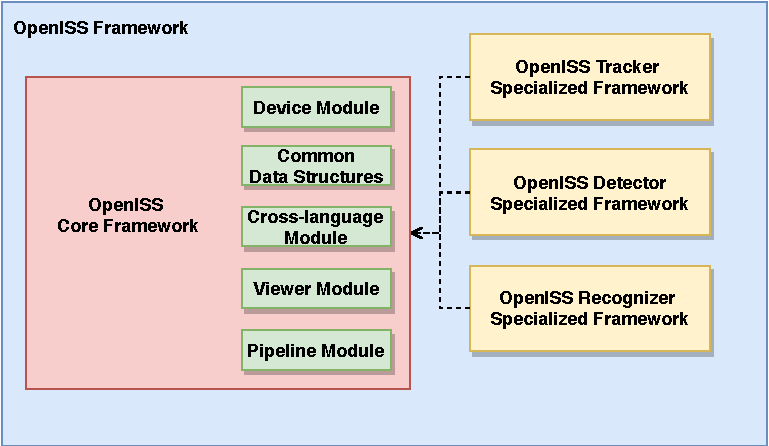
\includegraphics[width=\linewidth]{figures/framework_core_module.pdf}
    \caption[Core components of OpenISS framework]
    {Core components of OpenISS framework, each box in green means the core
    framework's frozen spot and each box in yellow represents a set of frozen
    spot of each specialized framework.}
    \label{fig:fw-core-module}
\end{figure}

In the following paragraphs, we are going to explain the design of each module 
within the core framework.

\subsection{Device Module}
\label{sec:fw-design-core-device}

Device module is one of the most essential modules in the whole OpenISS
framework because it is the lowest layer from our framework's point of view. It
is designed directly on top of the hardware drivers from various device
manufacturers.
Our design goal for this module is that we would like to block the physical
differences of cameras accessing them via a set of common APIs. Also, the
design should allow us to add support to more kinds of cameras easily without
changing the frozen spots itself.

With those requirements in mind, we found that one possible solution is to make
use of the polymorphism feature and dynamic dispatch mechanism, accessing the
subclass's method via a reference of its superclass. So what we need to do
will be just to come up with an elaborate abstraction that can be applied to
most of the common devices. After overall consideration, our design for the device
module shown as \autoref{fig:fw-core-device}. Since it is a core module, we are
going to explain some of these important abstract methods defined
in \texttt{OIDevice} class:

\begin{itemize}
    \item \texttt{rawDevice}: Sine our device model need to depend on
    the hardware driver, sometimes we may want to access the original device
    object created by the driver, this method is designed for it.

    \item \texttt{init}: This should contain the logic used to initialize
    the device, usually we need to call the driver's \texttt{init} method.

    \item \texttt{open}: This method is used for opening the device, it
    should be called after \texttt{init} method.

    \item \texttt{close}: This method is used for closing the device
    logically, most of the time we will release the resources which are not
    needed anymore.

    \item \texttt{enable}: This method is a shortcut for the following
    three specific enable methods.

    \item \texttt{enableColor}: This method tells the device to enable
    the color data stream.

    \item \texttt{enableDepth}: This method tells the device to enable
    the depth data stream.

    \item \texttt{enableRegistered}: This method tells the device to
    enable the registered data (infrared image data, aka. IR data) stream.

    \item \texttt{getIntrinsic} and \texttt{getExtrinsic}:
    These two methods are designed to obtain the intrinsic or extrinsic matrix
    respectively of the device if they are provided by the hardware driver.

    \item \texttt{getDepthScale}: This method is used to get the depth
    scale value which multiplies the depth data value can get the distance of
    in meter or centimeter.

    \item \texttt{readFrame(StreamType type)}: This method is the
    most important one, it is used to get a frame of data respect to the stream
    type (color, depth or IR) specified by the parameter.
\end{itemize}

\begin{figure}
    \centering
    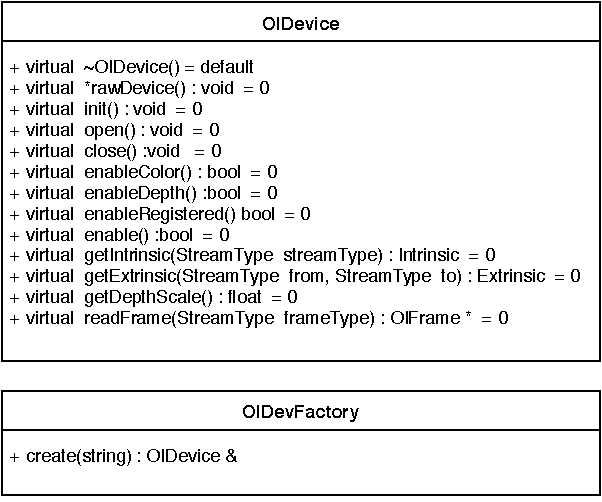
\includegraphics[scale=0.8]{figures/framework_core_device.pdf}
    \caption{Design of device module within OpenISS core framework.}
    \label{fig:fw-core-device}
\end{figure}

\subsection{Cross-Language Module}
\label{sec:fw-design-core-cross-lang}

As mentioned in \autoref{sec:related_work_obj_det} and
\autoref{sec:related_work_re_id}, the research community of both 
object detection and person re-identification have been dominated by deep 
learning approach since 2012.
Nowadays most of the available deep learning frameworks provide Python APIs for
convenient purpose, even though themselves were written in C/C++, developing
deep learning program directly using low-level APIs makes the works tedious and
problematic.
In order to address this issue, we design a cross-language module shown as
\autoref{fig:fw-core-cross-lang} which
enable the user to separate deep learning oriented program development from the
normal programming task. Our OpenISS framework itself is written in C/C++ (the
reason will be explained later in \autoref{sec:fw-inst-impl}), but for the deep
learning-based
models, we decide to develop them in Python then provide an encapsulated
internal API to invoke Python model from C/C++ by employing CPython introduced
in \autoref{sec:related_work_cpython}. It can not only help us to decouple the
framework's functionalities but also make good use of the existing community
resources.

\begin{figure}
    \centering
    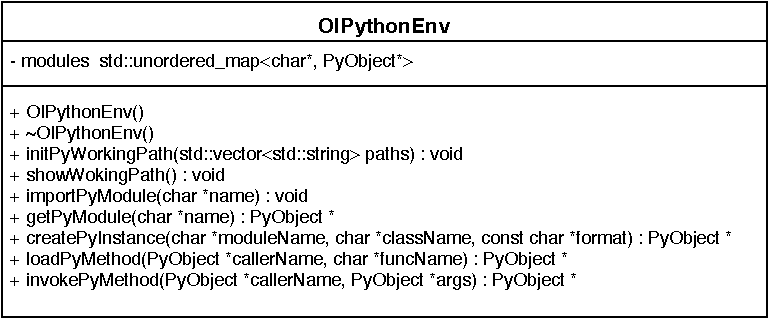
\includegraphics[scale=0.8]{figures/framework_core_cross_lang.pdf}
    \caption{Design of cross-language module within OpenISS core framework.}
    \label{fig:fw-core-cross-lang}
\end{figure}

The \texttt{OIPyhonEnv} is not an abstract class,
%class but a concrete one so
%that by definition it cannot be counted as frozen spot of the framework.
the reason why we put it under the core framework is that it actually serves as
an infrastructure even though the classes which will invoke the Python code
don't need to inherit from it but they have to use it as a dependency.
The \texttt{OIPythonEnv} class is used to encapsulate a Python script, four
core functions \texttt{initPyWorkingPath}, \texttt{createPyInstance},
\texttt{loadPyMethod} and \texttt{invokePythonMethod} are respectively used to
add a given path to the Python interpreter as a working path (Python will search
the requested module under all the working paths), create an object of a given
class which is visible within the encapsulated Python script, load (without
executing) the handler of a specified method which is visible from that file and
invoke a loaded function using its handler.

The design and usage philosophy of this module can be illustrated by
\autoref{fig:fw-core-cross-lang2}. Each instance of \texttt{OIPythonEnv}
can be used to represent a Python file (the box in green), a framework
developer trained, in our case, a deep learning model in Python (the red box)
and would like to expose some of the functionalities of it to the framework
users. Then they can write a C/C++ wrapper (the blue box) for it which
contains a member variable of type \texttt{OIPythonEnv} instantiated by the
names of classes and functions would like to expose. The framework users then
can use the Python code via our framework without knowing anything about Python
under the hood.

\begin{figure}
    \centering
    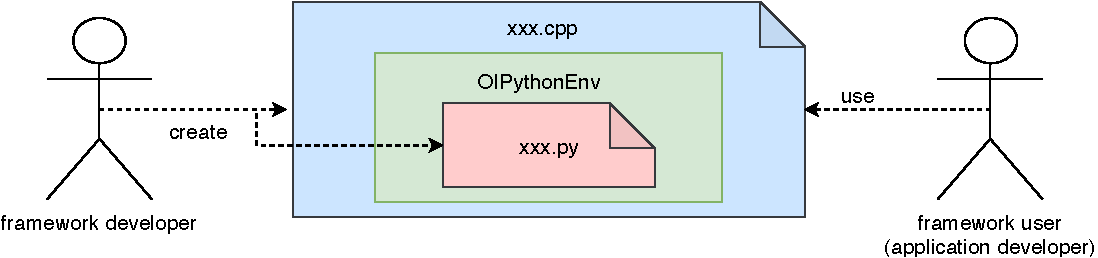
\includegraphics[scale=0.8]{figures/framework_core_cross_lang2.pdf}
    \caption
    {Usage scenario of the cross-language module of OpenISS core framework.}
    \label{fig:fw-core-cross-lang2}
\end{figure}

\subsection{Pipeline Module}
\label{sec:fw-design-core-pipeline}

\begin{figure}
    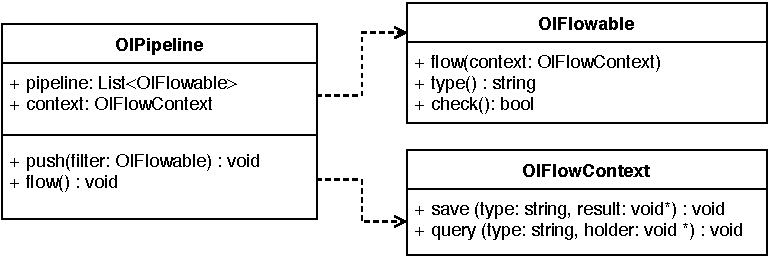
\includegraphics[width=\linewidth]{figures/framework_core_pipeline.pdf}
    \caption{The design of the pipeline module in the core framework.}
    \label{fig:fw-core-pipeline-uml}
\end{figure}

The pipeline module, as its name implies, provides a pipeline execution
mechanism for the framework users. It allows the user to chain multiple
filters together that the former's output will become the 
latter's input (no need the right before/after one).
When all these filters finish execution, we can achieve some specific goal, for
example, our final goal, tracking person across multiple cameras (detail will
be explained in \autoref{chap:fw-app}).

The design of the module can be described by the UML diagram shown as
\autoref{fig:fw-core-pipeline-uml}. The \texttt{OIPipeline} class contains a
list of filters and a reference with type \texttt{OIFlowContext} which is an
abstract class used to define the save and query behaviors of the temporary
result generated by the intermediate filters. The \texttt{push} method is used
to add a concrete filter into the pipeline while the \texttt{flow} method is the
switch to trigger the pipeline execution process.
The component which would like to serve as a filter must agree with the
\texttt{OIFlowable} contract. There are three functions defined within this
interface:

\begin{itemize}
    \item \texttt{flow}: It takes a reference of \texttt{OIFlowContext} as
    parameter, basically what this function does is calling the real logic
    method. For example, the \texttt{flow} function will call the
    \texttt{readFrame} function within \texttt{OIDevice}, the \texttt{detect}
    function within \texttt{OIDetector} and the \texttt{predict} function
    within \texttt{OIRecognizer}.

    \item \texttt{type}: It just returns the type of the filter itself, we may
    need it to differentiate some operations for various filters.

    \item \texttt{check}: It usually gets called before \texttt{flow} method,
    we perform necessary checking step here to ensure all the needed data are
    available before \texttt{flow} get executed.
\end{itemize}

The control flow of the pipeline module can be expressed by
\autoref{algo:fw-pipeline-flow} and the workflow can be visualized by
\autoref{fig:fw-core-pipeline}. With the \texttt{OIPipeline} class
definition in mind, there are two fields: \texttt{pipeline} which is a list of
filters and \texttt{context} which is actually a temporary data holder.
What we eventually do is that we loop over all the filters within the list and
invoke their \texttt{flow} method which is implemented in the concrete
classes and store the result in the concrete implementation of the
\texttt{OIFlowContext} class.
Inside the abstract \texttt{OIFlowContext} class, we define two methods:
\texttt{query(name:string, data:void*)} and \texttt{save(name:string,
data:void*)}. The method \texttt{query} is used to lookup the needed input
which output by the preceding for current executing filter while the
\texttt{save} function is used to save the temporary result generated by
the current filter. If there is more than one input or output from the current state,
we just need to call these two functions multiple times so we don't limit
ourselves to the number of input and output of a filter.

\begin{algorithm}
    \ForEach{filter in pipeline}{
        canFlow = filter.check(context)\;
        \If{canFlow}{
            result = filter.flow(context)\;
            context.save(filter.type(), result)\;
        }
    }
    \caption{The \texttt{flow} function within \texttt{OIPipeline} class}
    \label{algo:fw-pipeline-flow}
\end{algorithm}

\begin{figure}
    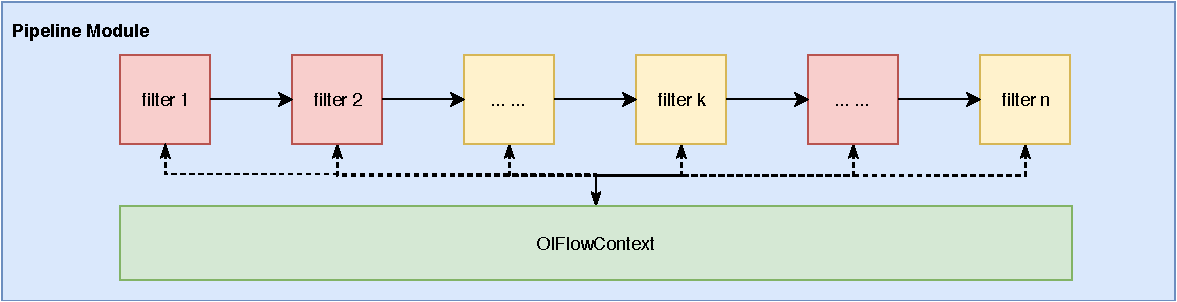
\includegraphics[width=\linewidth]{figures/framework_core_pipeline2.pdf}
    \caption{The design of the pipeline module in the core framework.}
    \label{fig:fw-core-pipeline}
\end{figure}

As you may notice the \texttt{OIPipeline} class, only have the method
\texttt{push} to allow the user to add filters but it doesn't provide any
removal interface for the existing filters which means each \texttt{OIPipeline}
instance is immutable. In other words, once it being defined you cannot change
its internal structure.
We design in such a way under the consideration that each pipeline instance is
used for a specific task. If you have more than one task then you will need to
reassemble a new pipeline instance and create another concrete
\texttt{OIFlowContext} object but you can reuse the same filter object if you
want. Also, all the filters reside in the pipeline are chained linearly. But
when you executing them, a conditional operation can be achieved by the
\texttt{check} method since it is the predecessor of the \texttt{flow} method.

\subsection{Common Data Structures}
\label{sec:fw-design-core-common-ds}

Common data structures, in OpenISS core framework, means these data structures
may be used by other modules within the core or cross multiple specialized
frameworks.
\texttt{OIFrame} is one of the most significant data structure of our
framework which is designed to represent the data captured by an input device
at a certain point of time. It will flow between the core and
specialized framework or even between several different specialized frameworks.
The design of \texttt{OIFrame} can be illustrated as
\autoref{fig:fw-core-oiframe}, the \texttt{OIFrame} is the highest level
abstraction provides the fundamental information of a frame. It has two
subclasses named \texttt{OIAbstractDataFrame} and \texttt{ICvImplFrame}, the
former is still an abstract class representing a frame contains data and the
latter is a concrete class describing a frame provided to the viewer.

\begin{figure}
    \centering
    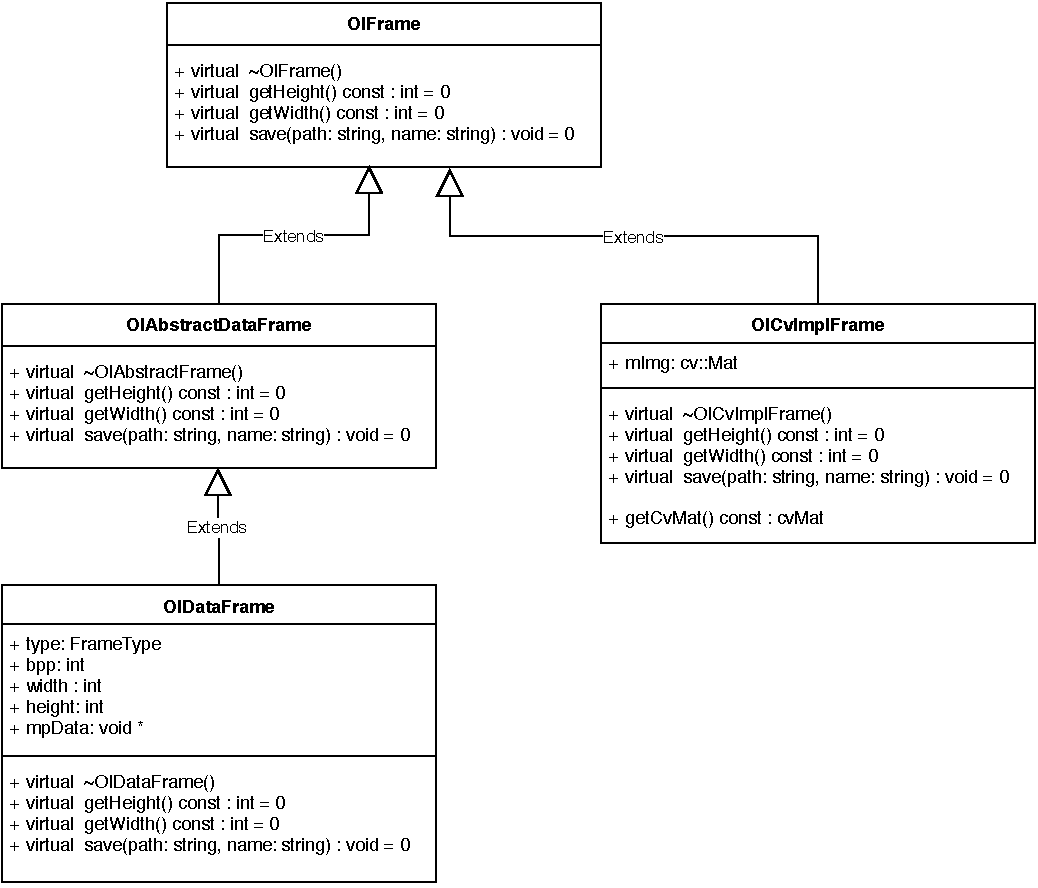
\includegraphics[width=\linewidth]{figures/framework_core_oiframe.pdf}
    \caption{
        Design of \texttt{OIFrame} inside common data structure within the core
        of OpenISS framework.
    }
    \label{fig:fw-core-oiframe}
\end{figure}

\subsection{Viewer Module}
\label{sec:fw-design-core-viewer}

The responsibility of the viewer module is straight forward and simple, as its name
implies, it is used for displaying the data for visualization purposes. Our
design for the viewer module is simple, as shown in
\autoref{fig:fw-core-viewer}, \texttt{OIViewer} is an abstract class which
contains a variable and a method. The variable \texttt{name} is an label used
to differentiate from various of displaying windows since the user may want to
show more than one frame, for example, show both color and depth image a the
same time.
The method \texttt{show} contains the logic for various libraries for
drawing. Currently, our framework only has one concrete implementation which
is \texttt{OIOpenCVViewer} based on the OpenCV library.
The \texttt{OIOpenGLViewer} was designed but it is still under
development.

\begin{figure}
    \centering
    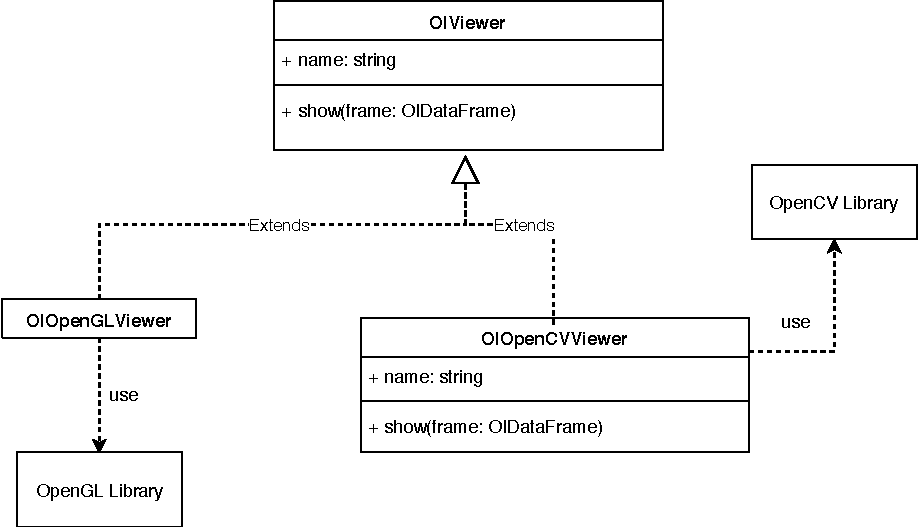
\includegraphics[scale=0.8]{figures/framework_core_viewer.pdf}
    \caption{Design of viewer module within the core of OpenISS framework.}
    \label{fig:fw-core-viewer}
\end{figure}

\section{Specialized Framework Design}
\label{sec:fw-design-spec}

% todo: 不应该讨论 chainable 这里,因为这些 specialized framework 不能 chain 在一起
The specialized framework is designed for solving a class of specific problems,
it provides a set of unified APIs to the framework users just like other
modules within the core framework but also defines the problem-specific data
structures and common methods. In an abstraction description, the data flow
within the framework can be viewed as \autoref{fig:fw-design-dataflow}. The raw
data from the physical device will firstly flow into the core of the framework
handling at least by the device module. Then these raw data will be wrapped to
become our OpenISS data structures and keep flowing into one or a pipeline of
specialized frameworks, since normally a large problem can be divided into
several subproblems, we believe that the combination of these specialized
frameworks may be able to solve more complex problems so we decide to make the
specialized framework chainable. Finally, the data will be converted into the
user's expected format and reaches to the end-user's application.

\begin{figure}
    \centering
    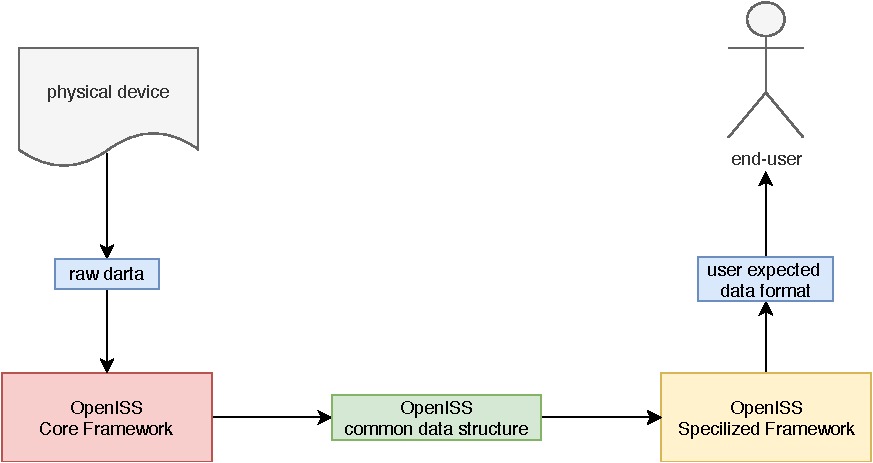
\includegraphics[scale=0.8]{figures/framework_dataflow.pdf}
    \caption{Data flow within the OpenISS framework.}
    \label{fig:fw-design-dataflow}
\end{figure}

In this thesis, we proposed three specialized frameworks, shown as the
rectangle in yellow in \autoref{fig:fw-core-module}. A combination of two
of them (detector and recognizer) aiming re-identify the same person across
multiple cameras in order to solve the limitation we mentioned in
\autoref{sec:intro-lim-issv2}.
And the other one (tracker) is used for skeleton tracking.
In this section, we will describe the architecture of each specialized
framework.
%and explain how the detector and recognizer can work together to
%achieve person ReID task.

\subsection{Tracker Specialized Framework Design}
\label{sec:fw-design-spec-tracker}

In \autoref{sec:intro-scen-req}, we explained the need for skeleton tracking.
Also, at the same time when this thesis is writing, there is another work
happening which aims at providing the functionality of gesture tracking. So it
is necessary for us to abstract the common methods of skeleton tracker, gesture
tracker and all other possible trackers.
Recall the problem a tracker attempt to address is that for a given sequence of
frames and a target, it is expected to locate the target for each of the
remaining frames.

In order to achieve that we design the tracker specialized framework shown as
\autoref{fig:fw-sub-tracker}. \texttt{OITrackerFactory} is responsible for
instantiating the concrete tracker object and tracker frame object.
\texttt{OITracker} is the abstract class of the tracker, it defines three basic
methods, \texttt{startTracking} for starting tracking, \texttt{stopTracking}
for stopping tracking and \texttt{readFrame} for reading data from the input
source and apply tracking algorithm on it that is where the magic should be
implemented in its subclass. The parameter, \texttt{OITrackerFrame}, acts as a
data container, the result of the tracking will be placed within this class and
it will be updated per frame time.

\begin{figure}
    \centering
    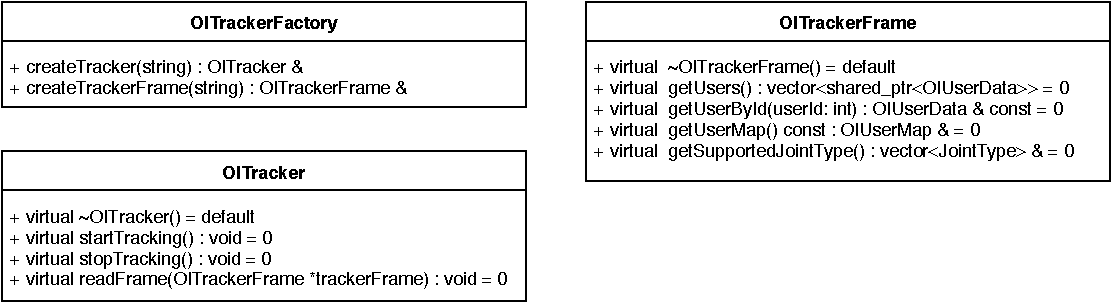
\includegraphics[width=\linewidth]{figures/framework_sub_tracker.pdf}
    \caption{Design of the OpenISS tracker specialized framework.}
    \label{fig:fw-sub-tracker}
\end{figure}

\subsection{Detector Specialized Framework Design}
\label{sec:fw-design-spec-detector}

As mentioned in \autoref{sec:intro-pbstat}, the ReID problem 
can be divided into two parts and one of them is object detection, so it is 
necessary to design a specialized framework for it. Since
we are designing a framework, in order to maintain its abstractness and
extensibility, we need to extract the common parts of different kinds of
detector then provide an abstraction of them.
Recap the definition of object detection we gave in \autoref{sec:intro-pbstat},
given an image $I$ and a list of objects $C$, the output will be a list of
bounding box $B$ which contains the instances of objects listed in $C$.

With such consideration, we design the specialized framework as
\autoref{fig:fw-sub-detector} shown. The \texttt{OIDetector} is the abstract
class which will be exposed to the user. Depends on the user's specific demand,
they can use either our pre-defined hot spot or create their own hot spot to
perform different kinds of detection algorithm. The frozen spot itself
\texttt{OIDetector} has a member variable \texttt{classList} contains the name
of the supported classes of a detector and a method named \texttt{detect} which
take an instance (hot spot) of the OpenISS common data structure
\texttt{OIFrame} as input and output a list of bounding boxes with the type
\texttt{OIBBox}.
Since the detector may be used to detect any kind of objects the shape of the
bounding box may be different. \texttt{OIBBox} is the abstract class of the
result which currently has two pre-defined hot spots \texttt{OIBBoxRect} and
\texttt{OIBBoxCircular} representing the rectangular and circular shape of
bounding box respectively. If any other shape is needed, the user can create
their own subclass inherited from the abstract class.
Finally, we adapt the factory pattern just like the device module to
encapsulate the creation process of different concrete detectors so that
the user just need to specify the name of the detector and pass it to a
factory's function named \texttt{create}. It will return a reference with type
\texttt{OIDetector} wrapping the desired concrete detector.

\begin{figure}
    \centering
    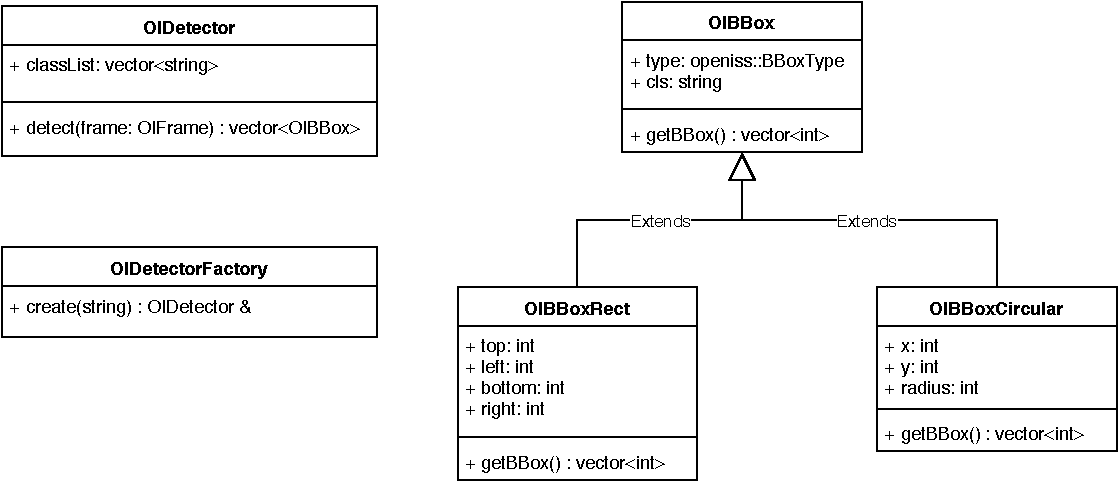
\includegraphics[width=\linewidth]{figures/framework_sub_detector.pdf}
    \caption{Design of the OpenISS detector specialized framework.}
    \label{fig:fw-sub-detector}
\end{figure}

\subsection{Recognizer Specialized Framework Design}
\label{sec:fw-design-spec-recognizer}

As mentioned in \autoref{sec:intro-pbstat}, ReID task can be divided
into two parts and we already explained object detection in the previous
section then the other one is object retrieval.
In other words, you are given a set of gallery images with their identities in
advanced. Then for a never seen query image, the recognizer is expected to tell
its identity among the gallery images.

Following the same pattern as the detector specialized framework, we design the
recognizer specialized framework shown as \autoref{fig:fw-sub-recognizer}.
Because we need to compare an item with all the items within a database, the
first step, of course, is that we need to create a database. According to our
definition, a database is a hashmap where the key is the identity string and
the value is a descriptor represented by the class \texttt{OIDescriptor}
computed from the source (e.g. an image or a video).
Inside the \texttt{OIDescriptor} class, the variable \texttt{srcPath} points to
the location of the source represented by this descriptor. The variable
\texttt{features} means the feature vector of the content of the source and the
variable \texttt{id} means the identity label.
Feature is one of the most significant parts for recognition, the core idea of
recognition is trying to find a way that can measure the distance between two
features accurately and effectively. Since these features are high dimensional
vectors, it is hard to imagine and tell what kinds of metrics can perform
better.
Feature is represented by the class \texttt{OINdArray} within the recognizer
specialized framework which encapsulates an N-dimensional array.
\texttt{OIRecognizerFactory} works exactly the same as its sibling within
the detector framework, we will omit the explanation for it here.
Finally, we reach the frozen spot of the recognizer representing by the class
named \texttt{OIRecognizer}. It has a variable name \texttt{database} which
holds all the pre-defined identities and three functions.
Method \texttt{attachDatabase} is easy to understand, as its name implies, it 
is used to attach the database to the recognizer.
Method \texttt{lookupDatabase} defines how to look up the possible result
with a given descriptor in hand among the database.
Method \texttt{predict} is one that user needs to invoke, it takes one 
parameter typed \texttt{OIFrame} which is the image contains the targeted item.

\begin{figure}
    \centering
    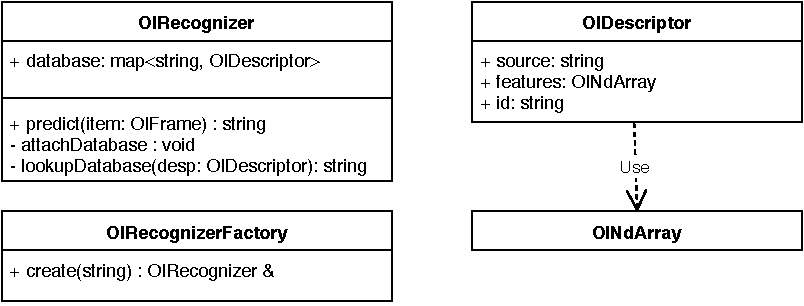
\includegraphics[scale=0.8]{figures/framework_sub_recognizer.pdf}
    \caption{Design of the OpenISS recognizer specialized framework.}
    \label{fig:fw-sub-recognizer}
\end{figure}

\section{Summary}
\label{sec:fw-design-summary}

In this chapter, we introduced the design of our framework. Began with why
we choose the framework solution. Followed by the way how we
structure the framework, we logically split the whole solution into two parts,
one sever as infrastructure called core framework and the other one is
responsible for specific tasks called specialized framework, in our design,
there can be multiple independent specialized frameworks.
Then we explained the design of each module (aka. frozen spot) within both the
core and specialized frameworks. In the next chapter, we are going to describe
how we create a framework instance to fulfill the requirements and scenarios
proposed in \autoref{sec:intro-scen-req}.

% EOF